\mysubsectionformatted{Design Principles e Design Patterns}
\myparagraph{
    In questa sezione si vanno ad analizzare i problemi che portano a un design
    inefficiente (Rotting Design).
    \\
    I sintomi sono i seguenti:
    \vspace{-0.5cm}
    \begin{center}
        \resizebox{\columnwidth}{!}{%
            \begin{tabular}{|
                    >{\columncolor[HTML]{3531FF}}l |l|}
                \hline
                {\color[HTML]{FFFFFF} \textbf{Rigidità}}   & \begin{tabular}[c]{@{}l@{}}Alta difficoltà nell'effettuare cambiamenti nel software, anche se si\\ tratta di cambiamenti semplici. Ogni cambiamento porta a sua volta la \\ necessità di cambiare ulteriori moduli dipendenti dal primo (effetto a cascata).\end{tabular}                                                                                    \\ \hline
                {\color[HTML]{FFFFFF} \textbf{Fragilità}}  & \begin{tabular}[c]{@{}l@{}}Tendenza del software di "rompersi" in seguito a dei cambiamenti nel software.\\ Spesso questi errori si verificano in aree che non hanno alcun collegamento\\ con l'area modificata.\end{tabular}                                                                                                                                \\ \hline
                {\color[HTML]{FFFFFF} \textbf{Immobilità}} & \begin{tabular}[c]{@{}l@{}}Non possibilità di riutilizzare il software da altri progetti oppure parti\\ dello stesso progetto.\end{tabular}                                                                                                                                                                                                                  \\ \hline
                {\color[HTML]{FFFFFF} \textbf{Viscosità}}  & \begin{tabular}[c]{@{}l@{}}Si distingue in viscosità del design e viscosità dell'ambiente (environment).\\ Il primo caso avviene se risulta facile commettere errori nel modificare il\\ design, a sua volta difficile nel fare le cose in modo corretto.\\ Il secondo caso avviene quando l'ambiente di sviluppo risulta lento e inefficiente.\end{tabular} \\ \hline
            \end{tabular}%
        }
    \end{center}
    Il fattore principale del perchè avvengono queste problematiche è dato dal fatto che al
    momento della creazione del design iniziale non vengono anticipati eventuali problemi.
    Il costante cambiamento delle parti del software porta a pensare che il design risulti
    inefficiente, quindi bisogna trovare un modo per renderlo più aperto al cambiamento.

    \mysubsubsectionformatted{Principi del Design Orientato agli Oggetti}
    \subsubsection{Open Closed Principle - OCP}
    \textit{Un modulo dovrebbe essere aperto alle estensioni ma chiuso per le modifiche}
    
    L'obiettivo di questo principio è garantire la creazione di moduli estendibili ma non senza modificare il codice sorgente.\\
    Si basa sulla tecnica dell'astrazione (in Java è abstract).
    
    \subsubsection{Liskov Substitution Principle - LSP}
    \textit{Le sottoclassi dovrebbero essere sostituibili per le loro classi base}
    
    L'obiettivo di questo principio è far sì che le classi derivate siano sostituibili per le loro classi padre. In questo modo,
    l'utente può continuare a usare le funzioni nonostante sia la classe derivata a essere passata (e non quella base).\\
    Sfortunatamente, qualora si violasse questo principio, risulterebbe difficile rilevare gli errori.
    
    \newpage
    \subsubsection{Dependency Inversion Principle - DIP}
    \textit{Si basa sull astrazione, non sulla concrezione}
    
    Questo principio si basa sull'uso delle interfacce o funzioni e classi astratte. Un'architettura orientata
    agli oggetti mostra una struttura dipendente dove la mggior parte delle dependency (relazioni) puntano verso
    le astrazioni. Nessuna dependency dovrebbe fare riferimento alle classi concrete. Il motivo è che gli oggetti concreti
    cambiano continuamente, quelli astratti meno frequentemente.
    
    \subsubsection{Interface Segregation Principle - ISP}
    \textit{Molte interfacce specifiche per gli utenti sono meglio di un'interfaccia generale}
    
    Se in una classe ci sono tanti clients, invece di caricare una classe con tutti i metodi richiesti dai clients, si
    creano delle interfacce specifiche per ciascuno. Nel caso più client necessitano dello stesso metodo, questo deve
    essere aggiunto in entrambi le interfacce.

    \mysubsubsectionformatted{Package Cohesion Principles}
    Sono utili per stabilire a quali package appartengono le classi.
    
    \subsubsection{Release Reuse Equivalency Principle - REP}
    \textit{La granulazione del riuso è la granulazione del rilascio}
    
    Spesso i client si rifiutano di utilizzare elementi a meno che gli autori non tengano traccia della versioni e
    mantengano le vecchie versioni per un po' di tempo. Quindi, un criterio per raggruppare le classi in un package è il riuso.
    Dal momento che i package sono delle unità di rilascio, a loro volta sono unità di riuso.
    
    \subsubsection{Common Closure Principle - CCP}
    \textit{Le classi che cambiano insieme sono inscindibili}
    
    Questo principio minimizza il numero di package che vengono cambiati per ogni rilascio del prodotto. Per far sì che
    questo principio funzioni, si raggruppano tutte quelle classi che pensiamo cambino insieme.
    
    \subsubsection{Common Reuse Principle - CRP}
    \textit{Classi che non vengono riusate insieme non dovrebbero essere raggruppate}

    Questo principio essenzialmente raggruppa quelle classi che non vengono usate insieme.
    
    \newpage
    \mysubsubsectionformatted{Package Coupling Principle}
    Questi principi governano le relazioni tra i package.
    \subsubsection{Acyclic Dependencies Principle - ADP}
    \textit{Le dipendenze tra i packages non devono creare dei cicli}

    Questo principio ha l'obiettivo di evitare la creazione di cicli, e quindi dipendenze cicliche, tra i package.
    L'eliminazione di un ciclo avviene in due modi, il primo consiste nel creare un nuovo package, il secondo è quello di
    usare i principi DIP e ISP.
    
    \subsubsection{Stable Dependencies Principle - SDP}
    \textit{Un modulo dovrebbe dipendere solo da moduli più stabili di lui}
    
    Quando si parla di \textit{stabilità} si intende il quantitativo di lavoro richiesto per effetturare una modifica.
    Esistono tanti fattori che rendono un software difficile da modificare (complessità, dimensione, chiarezza ecc\dots), ma
    fattori più importante è il fatto che tanti package software dipendano da uno solo.
    
    Esistono delle \coloredtext[blue]{\textbf{Metriche di Stabilità}} per semplificare le modifiche.
    \begin{center}
        \resizebox{\columnwidth}{!}{%
            \begin{tabular}{|
                    >{\columncolor[HTML]{3166FF}}l |l|}
                \hline
                {\color[HTML]{FFFFFF} \textbf{Ca - Afferent Coupling}} & \begin{tabular}[c]{@{}l@{}}Numero di classi fuori dal package che dipende dalle\\ classi dentro al package.\end{tabular}                 \\ \hline
                {\color[HTML]{FFFFFF} \textbf{Ce - Efferent Coupling}} & \begin{tabular}[c]{@{}l@{}}Numero di classi fuori dal package dipese dalle\\ classi dentro al package.\end{tabular}                      \\ \hline
                {\color[HTML]{FFFFFF} \textbf{I - Instability}}        & \begin{tabular}[c]{@{}l@{}}$I = \frac{Ce}{Ca + Ce}$\\ Se I = 0, il package è stabile,\\ altrimenti I = 1 ed è instabile.\end{tabular} \\ \hline
            \end{tabular}%
        }
    \end{center}

    \subsubsection{Stable Abstraction Principle - SAP}
    \textit{Package stabili dovrebbero essere astratti}
    \\
    Solitamente, una struttura di package prevede che quelli più in alto siano instabili e flessibili (facili da cambiare),
    mentre quelli più in basso sono difficili da cambiare per la loro stabilità.
    \\
    Un modo per rendere più semplice la modifica avviene tramite \coloredtext[blue]{\textbf{Metriche di Astrazione}}:
    \vspace{0.1cm}
    \begin{center}
        \resizebox{0.7\columnwidth}{!}{%
            \begin{tabular}{|
                    >{\columncolor[HTML]{3166FF}}l |l|}
                \hline
                {\color[HTML]{FFFFFF} \textbf{Nc}} & Numero di classi nel package.                                                                                                                                                 \\ \hline
                {\color[HTML]{FFFFFF} \textbf{Na}} & Numero di classi astratte nel package                                                                                                                                         \\ \hline
                {\color[HTML]{FFFFFF} \textbf{A}}  & \begin{tabular}[c]{@{}l@{}}Astrazioni, $A = \frac{Na}{Nc}$\\ Se A = 0, il package non ha classi astratte,\\ altrimenti A = 1 e contiene classi astratte.\end{tabular} \\ \hline
            \end{tabular}%
        }
    \end{center}

    \newpage
    Adesso possiamo confrontare le due metriche \textit{I} e \textit{A}. La metrica \textit{I} dovrebbe incrementare mentre
    \textit{A} decrementa, in questo modo, i package concreti dovrebbero essere instabili mentre quelli astratti dovrebbero
    essere stabili.
    \begin{center}
        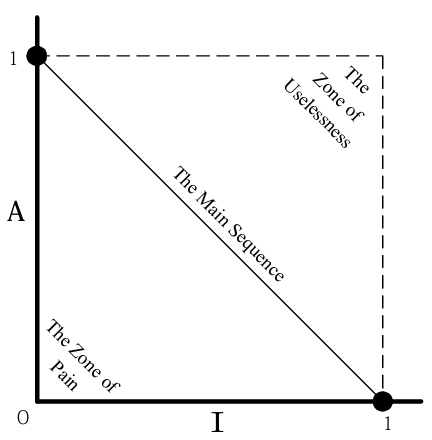
\includegraphics[scale=0.5]{design_principles_design_patterns/Grafo_AvsI.jpeg}
    \end{center}
    Nel grafico, in alto a sinistra troviamo i package astratti e stabili, in basso a destra i package concreti e instabili.
    \\
    Altre metriche utili sono le \coloredtext[blue]{\textbf{Metriche di Distanza}}, utili per stabilire quanto è lontano
    un package dalla \textit{main sequence}, ovvero la distanza massima tra i package concreti e quell astratti.
    \begin{center}
        \resizebox{\columnwidth}{!}{%
            \begin{tabular}{|
                    >{\columncolor[HTML]{3166FF}}l |l|}
                \hline
                {\color[HTML]{FFFFFF} \textbf{D - Distance}}             & $D = \frac{|A + I - 1|}{\sqrt{2}}$ \\ \hline
                {\color[HTML]{FFFFFF} \textbf{D' - Normalized Distance}} & \begin{tabular}[c]{@{}l@{}}$D' = |A + I - 1|$\\ Se D' = 0, il package è nella main sequence,\\ se D' = 1, è il più lontano possibile.\end{tabular} \\ \hline
            \end{tabular}%
        }
    \end{center}
    \newpage

}